\documentclass[letterpaper]{report}

%Falta agregar Anexos de tablas y la bibliografia

\usepackage{graphicx}
\usepackage[latin1]{inputenc}
\usepackage[spanish,es-tabla]{babel}
\usepackage{graphicx} %Permite exportar imagenes en formato eps
\usepackage{url} %Tipo de fuente para correos y paginas
\usepackage{pgf}
\usepackage{fleqn}
\usepackage{amssymb}
\usepackage{amsmath}
\usepackage{fancyvrb}
\usepackage{sectsty}
\usepackage{makeidx}
\usepackage{colortbl} %Permite colocar colores a las tablas
\usepackage{booktabs}
\usepackage[final]{pdfpages}
\usepackage{fancyhdr}
\usepackage{color}   %May be necessary if you want to color links
\usepackage{hyperref}
\usepackage{listings}
\lstset{ %
  language=Python
  }



\pagestyle{fancy}
\fancyhf{}
%\renewcommand{\headrulewidth}{0pt} % optional
\fancyhead[L]{\nouppercase{\leftmark}}
\fancyhead[R]{}
\fancyfoot[RO, LE] {\thepage}
\renewcommand{\footrulewidth}{0.4pt}

\begin{document}
%%%%%%%%%%%%%%%%%%%%%%%%%%
%Definici�n de la portada%
%%%%%%%%%%%%%%%%%%%%%%%%%%
\begin{titlepage}
    \begin{center}
	    
\includegraphics[width=8cm]{Imagenes/logoutfsm.png}
	
	   \begin{center}
		\Large{\sc{Departamento de Inform�tica}}\\
		\large{\sc{Valpara�so - Chile}}\\	
	    \end{center}
\begin{center}
\line(1,0){100}
\end{center}
\vspace{1cm}
	\begin{center}
		\textbf{\huge{An�lisis de herramientas para mejorar el desarrollo de aplicaciones Android}}
	\end{center}

	\vspace{1cm}
	\begin{center}
		\large{\sc{Cristopher Nicol�s Oyarz�n Altamirano}}
	\end{center}
    \vspace{2cm}
	\begin{center}
         	\normalsize{Memoria de titulaci�n para optar al T�tulo de:}
            \normalsize{\sc{\\INGENIERO CIVIL INFORM�TICO}}
	\end{center}
 \vspace{1cm}
 \begin{center}
		\large{Profesora Gu�a: Cecilia Reyes\\}
		\large{Profesor Correferente: Chihau Chau\\}
	\end{center}
	
\end{center}

\vspace{1cm}
\begin{center}
 \normalsize{\sc{Abril del 2014.}}\\
\end{center}

	
\end{titlepage} 

\newpage{\pagestyle{empty}\cleardoublepage}

\section*{Agradecimientos}

Agradezco a Lorem ipsum ad his scripta blandit partiendo, eum fastidii accumsan euripidis in, eum liber hendrerit an. Qui ut wisi vocibus suscipiantur, quo dicit ridens inciderint id. Quo mundi lobortis reformidans eu, legimus senserit definiebas an eos. Eu sit tincidunt incorrupte definitionem, vis mutat affert percipit cu, eirmod consectetuer signiferumque eu per. In usu latine equidem dolores. Quo no falli viris intellegam, ut fugit veritus placerat per.

Ius id vidit volumus mandamus, vide veritus democritum te nec, ei eos debet libris consulatu. No mei ferri graeco dicunt, ad cum veri accommodare. Sed at malis omnesque delicata, usu et iusto zzril meliore. Dicunt maiorum eloquentiam cum cu, sit summo dolor essent te. Ne quodsi nusquam legendos has, ea dicit voluptua eloquentiam pro, ad sit quas qualisque. Eos vocibus deserunt quaestio ei. 

\newpage
\section*{Resumen}

El crecimiento que ha tenido el sistema operativo Android es considerable. Existen m�s de un mill�n de aplicaciones disponibles en la tienda de Google y cada mes este n�mero se ve incrementado. Es por ello que el proceso de desarrollo de aplicaciones ha ganado vital importancia. El objetivo de esta memoria es estudiar y comparar herramientas que ayuden a mejorar el desarrollo de aplicaciones Android de tal manera de proveer a los desarrolladores una gu�a pr�ctica que les permita tomar mejores decisiones en el transcurso de un proyecto.

Lorem ipsum ad his scripta blandit partiendo, eum fastidii accumsan euripidis in, eum liber hendrerit an. Qui ut wisi vocibus suscipiantur, quo dicit ridens inciderint id. Quo mundi lobortis reformidans eu, legimus senserit definiebas an eos. Eu sit tincidunt incorrupte definitionem, vis mutat affert percipit cu, eirmod consectetuer signiferumque eu per. In usu latine equidem dolores. Quo no falli viris intellegam, ut fugit veritus placerat per.

\section*{Summary}
Ius id vidit volumus mandamus, vide veritus democritum te nec, ei eos debet libris consulatu. No mei ferri graeco dicunt, ad cum veri accommodare. Sed at malis omnesque delicata, usu et iusto zzril meliore. Dicunt maiorum eloquentiam cum cu, sit summo dolor essent te. Ne quodsi nusquam legendos has, ea dicit voluptua eloquentiam pro, ad sit quas qualisque. Eos vocibus deserunt quaestio ei. 

\tableofcontents

\chapter{Introducci�n}

\section{Definici�n del Problema}

Android es una sistema operativo emergente de c�digo abierto, dise�ado especialmente para dispositivos m�viles, el cual fue presentado el a�o 2007. El crecimiento que ha tenido los �ltimos a�os ha sido considerable, dominando el mercado ampliamente, existiendo m�s de mil millones de dispositivos activados en todo el mundo.

El gran problema que ha tenido que enfrentar la gente que desarrolla aplicaciones para  Android es la fragmentaci�n generada por la inmensa cantidad y variedad de dispositivos existentes, entre los que se encuentran smartphones, notebooks, netbooks, tablets, televisores, etc. Adem�s, existen variadas versiones del mismo sistema operativo en uso. Esto conlleva muchos problemas a la hora de dise�ar y desarrollar aplicaciones ya que es imposible poder probar nuestra aplicaci�n en cada uno de los dispositivos para los cuales estar� disponible, por lo que lo m�s probable es que existir�n problemas de interfaz gr�fica si no estamos listos para soportar variadas resoluciones de pantallas. Tambi�n es necesario tener un buen sistema de reporte de crashes ya que muchas veces, por m�s que nuestro c�digo funcione de forma correcta en un dispositivo con Android 4.3, en el mismo dispositivo con Android 4.0.4 se puede comportar de forma distinta. Si bien, estos son s�lo algunos de los problemas que se deben enfrentar, existen otros m�s, tales como: la distribuci�n de versiones alphas y betas, tracking de eventos, mejoras de performance, testing, etc. 

Hoy en d�a existen variadas herramientas que ayudan a afrontar muchos de estos problemas. El r�pido crecimiento de Android ha estado acompa�ado de la aparici�n de una gran cantidad de librer�as y proyectos opensource con diversas soluciones. Estas herramientas se dan a conocer a trav�s de las redes sociales o comunidades de programadores. Debido a que estas librer�as se encuentran dispersas es dif�cil saber cual de todas elegir, ya que se desconocen los pros y contras de cada una de ellas. Esto provoca que muchas veces, por desconocimiento o falta de tiempo, no se realice una decisi�n informada y se use la primera librer�a encontrada.

Lorem ipsum ad his scripta blandit partiendo, eum fastidii accumsan euripidis in, eum liber hendrerit an. Qui ut wisi vocibus suscipiantur, quo dicit ridens inciderint id. Quo mundi lobortis reformidans eu, legimus senserit definiebas an eos. Eu sit tincidunt incorrupte definitionem, vis mutat affert percipit cu, eirmod consectetuer signiferumque eu per. In usu latine equidem dolores. Quo no falli viris intellegam, ut fugit veritus placerat per.

Ius id vidit volumus mandamus, vide veritus democritum te nec, ei eos debet libris consulatu. No mei ferri graeco dicunt, ad cum veri accommodare. Sed at malis omnesque delicata, usu et iusto zzril meliore. Dicunt maiorum eloquentiam cum cu, sit summo dolor essent te. Ne quodsi nusquam legendos has, ea dicit voluptua eloquentiam pro, ad sit quas qualisque. Eos vocibus deserunt quaestio ei.

Lorem ipsum ad his scripta blandit partiendo, eum fastidii accumsan euripidis in, eum liber hendrerit an. Qui ut wisi vocibus suscipiantur, quo dicit ridens inciderint id. Quo mundi lobortis reformidans eu, legimus senserit definiebas an eos. Eu sit tincidunt incorrupte definitionem, vis mutat affert percipit cu, eirmod consectetuer signiferumque eu per. In usu latine equidem dolores. Quo no falli viris intellegam, ut fugit veritus placerat per.

Ius id vidit volumus mandamus, vide veritus democritum te nec, ei eos debet libris consulatu. No mei ferri graeco dicunt, ad cum veri accommodare. Sed at malis omnesque delicata, usu et iusto zzril meliore. Dicunt maiorum eloquentiam cum cu, sit summo dolor essent te. Ne quodsi nusquam legendos has, ea dicit voluptua eloquentiam pro, ad sit quas qualisque. Eos vocibus deserunt quaestio ei.

Lorem ipsum ad his scripta blandit partiendo, eum fastidii accumsan euripidis in, eum liber hendrerit an. Qui ut wisi vocibus suscipiantur, quo dicit ridens inciderint id. Quo mundi lobortis reformidans eu, legimus senserit definiebas an eos. Eu sit tincidunt incorrupte definitionem, vis mutat affert percipit cu, eirmod consectetuer signiferumque eu per. In usu latine equidem dolores. Quo no falli viris intellegam, ut fugit veritus placerat per.

Ius id vidit volumus mandamus, vide veritus democritum te nec, ei eos debet libris consulatu. No mei ferri graeco dicunt, ad cum veri accommodare. Sed at malis omnesque delicata, usu et iusto zzril meliore. Dicunt maiorum eloquentiam cum cu, sit summo dolor essent te. Ne quodsi nusquam legendos has, ea dicit voluptua eloquentiam pro, ad sit quas qualisque. Eos vocibus deserunt quaestio ei.

\section{Objetivos}
Lorem ipsum ad his scripta blandit partiendo, eum fastidii accumsan euripidis in, eum liber hendrerit an. Qui ut wisi vocibus suscipiantur, quo dicit ridens inciderint id. Quo mundi lobortis reformidans eu, legimus senserit definiebas an eos. Eu sit tincidunt incorrupte definitionem, vis mutat affert percipit cu, eirmod consectetuer signiferumque eu per. In usu latine equidem dolores. Quo no falli viris intellegam, ut fugit veritus placerat per.

\subsection{Objetivo principal}
\begin{itemize}
\item Estudiar y comparar herramientas que ayudan a mejorar el desarrollo de aplicaciones Android de tal manera de proveer a los desarrolladores una gu�a pr�ctica que les permita tomar mejores decisiones en el transcurso de un proyecto.

\end{itemize}

\subsection{Objetivos espec�ficos}
\begin{itemize}
\item Identificar los distintos problemas existentes durante el desarrollo de aplicaciones Android.

\item Estudiar y clasificar las herramientas actuales en base a los distintos problemas que buscan solucionar.

\item Realizar un an�lisis comparativo para cada una de las categorias elegidas.

\item Implementar las mejores herramientas en un entorno real de desarrollo.
\end{itemize}

\section{Estructura del documento}

Lorem ipsum ad his scripta blandit partiendo, eum fastidii accumsan euripidis in, eum liber hendrerit an. Qui ut wisi vocibus suscipiantur, quo dicit ridens inciderint id. Quo mundi lobortis reformidans eu, legimus senserit definiebas an eos. Eu sit tincidunt incorrupte definitionem, vis mutat affert percipit cu, eirmod consectetuer signiferumque eu per. In usu latine equidem dolores. Quo no falli viris intellegam, ut fugit veritus placerat per.

Ius id vidit volumus mandamus, vide veritus democritum te nec, ei eos debet libris consulatu. No mei ferri graeco dicunt, ad cum veri accommodare. Sed at malis omnesque delicata, usu et iusto zzril meliore. Dicunt maiorum eloquentiam cum cu, sit summo dolor essent te. Ne quodsi nusquam legendos has, ea dicit voluptua eloquentiam pro, ad sit quas qualisque. Eos vocibus deserunt quaestio ei.

Lorem ipsum ad his scripta blandit partiendo, eum fastidii accumsan euripidis in, eum liber hendrerit an. Qui ut wisi vocibus suscipiantur, quo dicit ridens inciderint id. Quo mundi lobortis reformidans eu, legimus senserit definiebas an eos. Eu sit tincidunt incorrupte definitionem, vis mutat affert percipit cu, eirmod consectetuer signiferumque eu per. In usu latine equidem dolores. Quo no falli viris intellegam, ut fugit veritus placerat per.

Ius id vidit volumus mandamus, vide veritus democritum te nec, ei eos debet libris consulatu. No mei ferri graeco dicunt, ad cum veri accommodare. Sed at malis omnesque delicata, usu et iusto zzril meliore. Dicunt maiorum eloquentiam cum cu, sit summo dolor essent te. Ne quodsi nusquam legendos has, ea dicit voluptua eloquentiam pro, ad sit quas qualisque. Eos vocibus deserunt quaestio ei.

Lorem ipsum ad his scripta blandit partiendo, eum fastidii accumsan euripidis in, eum liber hendrerit an. Qui ut wisi vocibus suscipiantur, quo dicit ridens inciderint id. Quo mundi lobortis reformidans eu, legimus senserit definiebas an eos. Eu sit tincidunt incorrupte definitionem, vis mutat affert percipit cu, eirmod consectetuer signiferumque eu per. In usu latine equidem dolores. Quo no falli viris intellegam, ut fugit veritus placerat per.

Ius id vidit volumus mandamus, vide veritus democritum te nec, ei eos debet libris consulatu. No mei ferri graeco dicunt, ad cum veri accommodare. Sed at malis omnesque delicata, usu et iusto zzril meliore. Dicunt maiorum eloquentiam cum cu, sit summo dolor essent te. Ne quodsi nusquam legendos has, ea dicit voluptua eloquentiam pro, ad sit quas qualisque. Eos vocibus deserunt quaestio ei. 

\newpage{\pagestyle{empty}\cleardoublepage}

\chapter{Estado del Arte}

\definecolor{dkgreen}{rgb}{0,0.6,0}
\definecolor{gray}{rgb}{0.5,0.5,0.5}
\definecolor{mauve}{rgb}{0.58,0,0.82}

\lstset{frame=tb,
  language=Java,
  aboveskip=3mm,
  belowskip=3mm,
  showstringspaces=false,
  columns=flexible,
  basicstyle={\small\ttfamily},
  numbers=none,
  numberstyle=\tiny\color{gray},
  keywordstyle=\color{blue},
  commentstyle=\color{dkgreen},
  stringstyle=\color{mauve},
  breaklines=true,
  breakatwhitespace=true
  tabsize=3
}

En este cap�tulo se dar� a conocer una breve descripci�n del sistema operativo Android. Se comenzar� con una introducci�n y se hablar� de sus inicios, su arquitectura y la evoluci�n que ha tenido con el tiempo. Adem�s se hablar� sobre los problemas m�s comunes al momento de comenzar a desarrollar una aplicaci�n para Android.
\section{Introducci�n a Android}
Android es un sistema operativo basado en Linux, dise�ado principalmente para dispositivos m�viles t�ctiles, tales como smartphones y tablets. A continuaci�n se dar�n a conocer algunos detalles sobre sus inicios, arquitectura y evoluci�n con el tiempo.
\subsection{Inicios de Android}
Android, Inc. fue fundada en Palo Alto, California en Octubre del 2003 por Andy Rubin, Rich Miner, Nick Sears and Chris White. Su objetivo era desarrollar dispositivos m�viles m�s inteligentes, que estuvieran m�s enfocados en la localizaci�n del due�o y en distintas preferencias.\\
\par
Google compr� a Android Inc. el 17 de Agosto del 2005. Poco se sab�a sobre esta compa��a para ese entonces ya que estuvo funcionando de forma secreta, sin dar a conocer muchos detalles sobre lo que desarrollaban. Muchos asum�an que Google estaba planeando entrar al mercado de dispositivos m�viles. De ahi en adelante los esfuerzos de Google se enfocaron en conversaciones con fabricantes y carriers, con la promesa de proveer de un sistema flexible y actualizable.\\
\par 
Sin embargo, la aparici�n del iPhone el 9 de Enero del 2007 tuvo un efecto disruptivo en el desarrollo de Android. Hasta el momento se contaba con un prototipo, el cu�l se acercaba m�s a lo que podr�a ser un tel�fono BlackBerry, sin pantalla t�ctil y con un teclado f�sico. Por lo que se comenz� inmediatamente un trabajo de reingenier�a del sistema operativa y del prototipo para que fuese capaz de competir con el iPhone.\\
\par
El 6 de Noviembre del 2007 fue fundada la Open Handset Alliance, una alianza comercial liderada por Google con compa��as tecnol�gicas como HTC, Sony y Samsung, operadores de carriers como Nextel y T-Mobile y fabricantes de chips, con el objetivo de desarrollar est�ndares abiertos para dispositivos m�viles. El primer smartphone disponible que funcionaba sobre Android fue el HTC Dream, lanzado el 22 de Octubre del 2008.
\subsection{Arquitectura}
La arquitectura del sistema Android, tambi�n llamado stack, se puede apreciar en la figura ~\ref{fig:Fig1} y est� compuesta por cuatro capas:
\begin{itemize}
\item \textbf{Kernel de Linux:} La capa m�s profunda es su n�cleo en Linux, un sistema operativo abierto, el cu�l es portable y seguro. Para cada pieza de hardware, como la c�mara o el bluetooth, existe un driver dentro del kernel, que permitir� a la capa superior hacer uso de ella, por lo que funciona como una capa de abstracci�n. El kernel adem�s se encarga de la gesti�n de los diversos recursos del dispositivo, como la energ�a o la memoria, elementos de comunicaci�n, procesos, etc.
\par
\item \textbf{Bibliotecas:} La segunda capa en el stack contiene bibliotecas nativas, las cu�les est�n escritas en C o C++, y son compiladas para la arquitectura espec�fica del dispositivo. En la mayor�a de los casos el fabricantes es quien se encarga de instalarla en su dispositivo. Las bibliotecas inclu�das en esta capa son: el motor gr�fico OpenGL, el sistema de gesti�n de base de datos SQLite, cifrado de comunicaciones SSL, motor de manejo de tipos de letra FreeType, entre otras.
\par
El entorno de ejecuci�n de Android tambi�n est� compuesto por bibliotecas, por lo que no se considera una capa. Debido a las limitaciones de los dispositivos en los que debe funcionar, Google decidi� crear la m�quina virtual Dalvik, que funciona de forma similar a la m�quina virtual de Java. Esta permite crear aplicaciones con un mejor rendimiento y menor consumo de energ�a, lo que es muy importante en dispositivos m�viles. Adem�s en el entorno de ejecuci�n se incluyen la mayor�a de las bibliotecas b�sicas de Java.

\begin{figure}[h!]
\centering
	    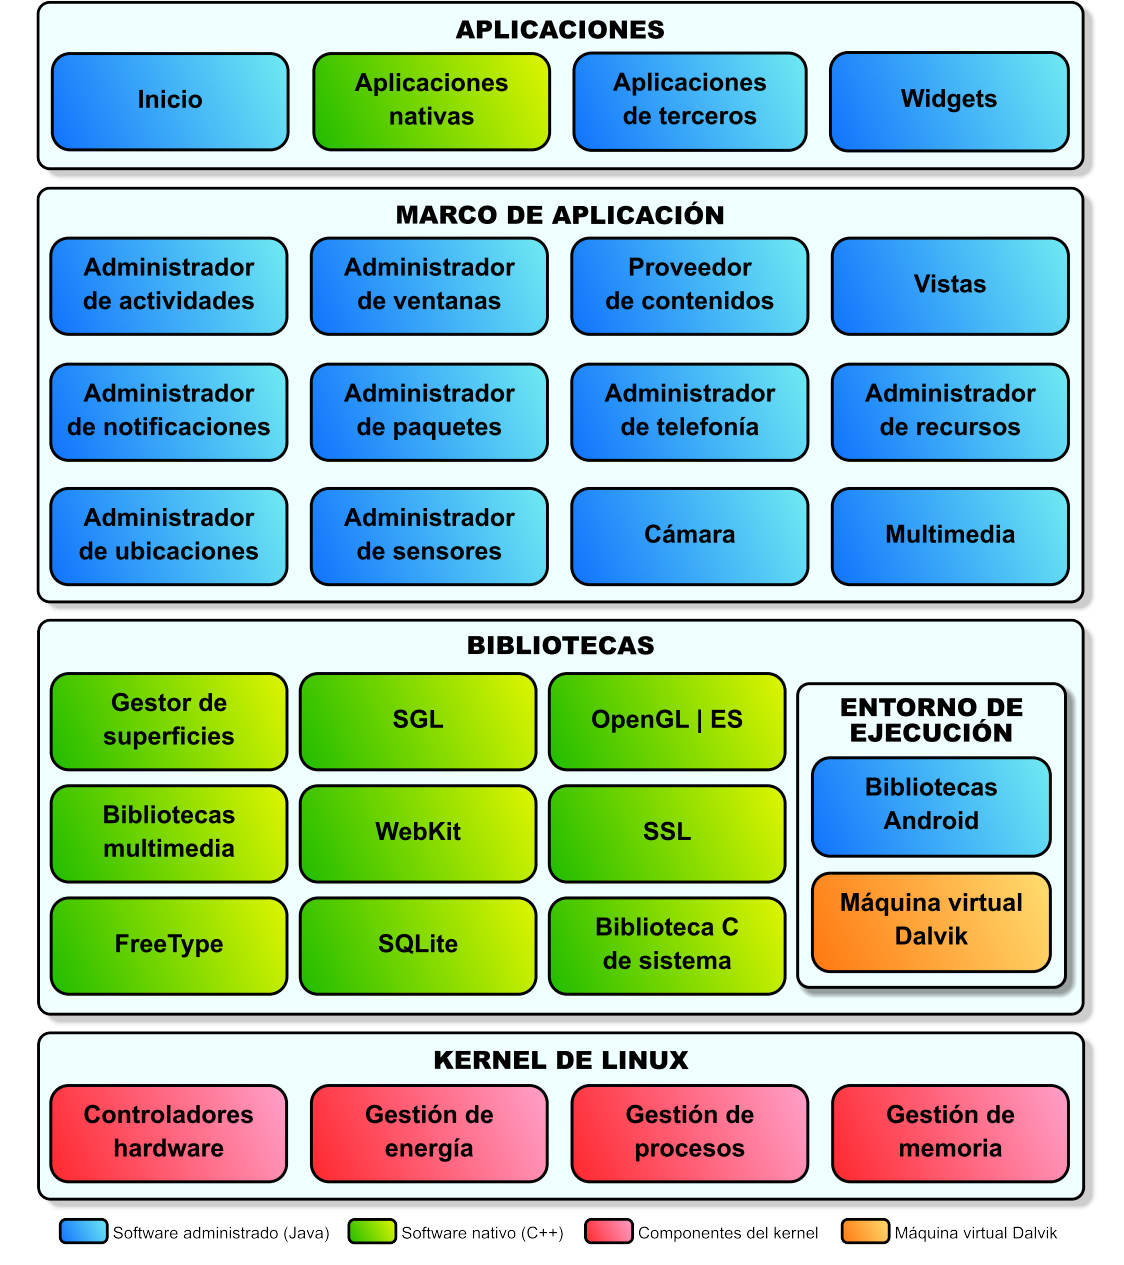
\includegraphics[width=12cm]{Imagenes/arquitectura_android}
\caption{Arquitectura de Android, compuesta por cuatro capas}
\label{fig:Fig1}
\end{figure}

\item \textbf{Marco o Framework de Aplicaciones:} La tercera capa est� compuesta por todas las clases y servicios que se utilizan al momento de programar aplicaciones. Los compontentes que posee son:
\begin{itemize}
\item \textbf{Administrado de actividades (Activity Manager):} Gestiona la pila de actividades de la aplicaci�n, como tambi�n su ciclo de vida.

\item \textbf{Administrador de ventanas (Windows Manager):} Organiza lo que se mostrar� en pantalla. Crea las superficies en la pantalla, que posteriormente estar�n ocupadas por las actividades.

\item \textbf{Proveedor de contenidos (Content Provider):} Encapsula los datos que pueden ser compartidos por las aplicaciones, facilitando la comunicaci�n entre estas.

\item \textbf{Vistas (Views):} Son los elementos que nos permitir�n construir las interfaces de usuario, como listas, botones, textos, hasta otros elementos m�s avanzados como visores de mapas.

\item \textbf{Administrador de notificaciones (Notification Manager):} Provee los servicios que notifican al usuario, mostrando alertas en la barra de estado. Tambi�n permite activar el vibrado, reproducir alertas de sonido y utilizar las luces del dispositivo.

\item \textbf{Administrador de paquetes (Package Manager):} Gestiona la instalaci�n de nuevos paquetes y adem�s permite obtener informaci�n sobre los que ya est�n instalados.

\item \textbf{Administrador de telefon�a (Telephony Manager):} Permite realizar llamadas, como tambi�n el env�o y recepci�n de SMS.

\item \textbf{Administrado de recursos (Resource Manager):} A trav�s de este administrador se podr� acceder a los elementos que no forman parte del c�digo, como im�genes, sonidos, layouts, etc. 

\item \textbf{Administrado de ubicaciones (Location Manager):} Permite obtener la posici�n geogr�fica actual del dispositivo a trav�s de GPS o redes.

\item \textbf{Administrado de sensores (Sensor Manager):} Permite la manipulaci�n de distintos sensores del dispositivo, como el aceler�metro, giroscopio, br�jula, sensor de proximidad, etc.

\item \textbf{C�mara:} Permite el uso de la c�mara del dispositivo para la obtenci�n de fotograf�as o v�deos.

\item \textbf{Multimedia:} Permite la visualizaci�n y reproducci�n de im�genes, v�deos y audio.

\end{itemize}

\item \textbf{Aplicaciones:} En esta capa se encuentran todas las aplicaciones del dispositivo, tanto las preinstaladas, como aquellas instaladas por el usuario. Tambi�n est� la aplicaci�n principal del sistema, el Inicio o launcher, desde donde se inician todas las aplicaciones.
\end{itemize}

\subsection{�C�mo las aplicaciones son compiladas?}
Al momento de desarrollar una aplicaci�n de Android, generalmente se crea un proyecto usando un IDE (\textit{Integrated Development Environment}) como Eclipse o Android Studio. El proyecto contendr� c�digo fuente en Java y recursos. Cuando se compila el proyecto lo que ocurre es que se generan los Bytecode Java (archivos .class) en base a nuestro c�digo fuente Java (archivos .java). Luego se compilan estos archivos .class a archivos ejecutables Dalvik (archivos .dex), los cuales pueden ser ejectuados por la m�quina virtual Dalvik que est� disponible en todos los dispositivos Android.\\
\par
Al compilar un proyecto se colocan los archivos .dex y el resto de los archivos del proyecto en un archivo llamadado APK (\textit{Android Package}). Este contiene todos los archivos necesarios para ejecutar la aplicaci�n, incluyendo los archivos .dex, recursos compilados, recursos sin compilar, y una versi�n binaria del Android manifest.\\
\par
El \textit{Android manifest} es un archivo que especifica informaci�n esencial que el sistema debe tener antes de ejecutar la aplicaci�n. Toda aplicaci�n debe tener este archivo de forma no binaria en su proyecto.\\
\par
Por razones de seguridad todas las aplicaciones de Android deben ser firmadas digitalmente con un certificado.\\
\par
Finalmente el \textit{Android debug bridge (ADB)} permiten que el IDE se comunique con un dispositivo f�sico de Android o un emulador.

\subsection{Tipos de dispositivos}
En el sitio web de Android \cite{1}, se pueden apreciar los dos tipos de dispositivos m�s populares de la plataforma, los smartphones y las tablets (Figura \ref{fig:Fig2}). Sin embargo, debido a que el c�digo de Android es de c�digo abierto, este puede ser personalizado para que funcione con otros tipos de dispositivos electr�nicos.

\begin{figure}[h!]
\centering
	    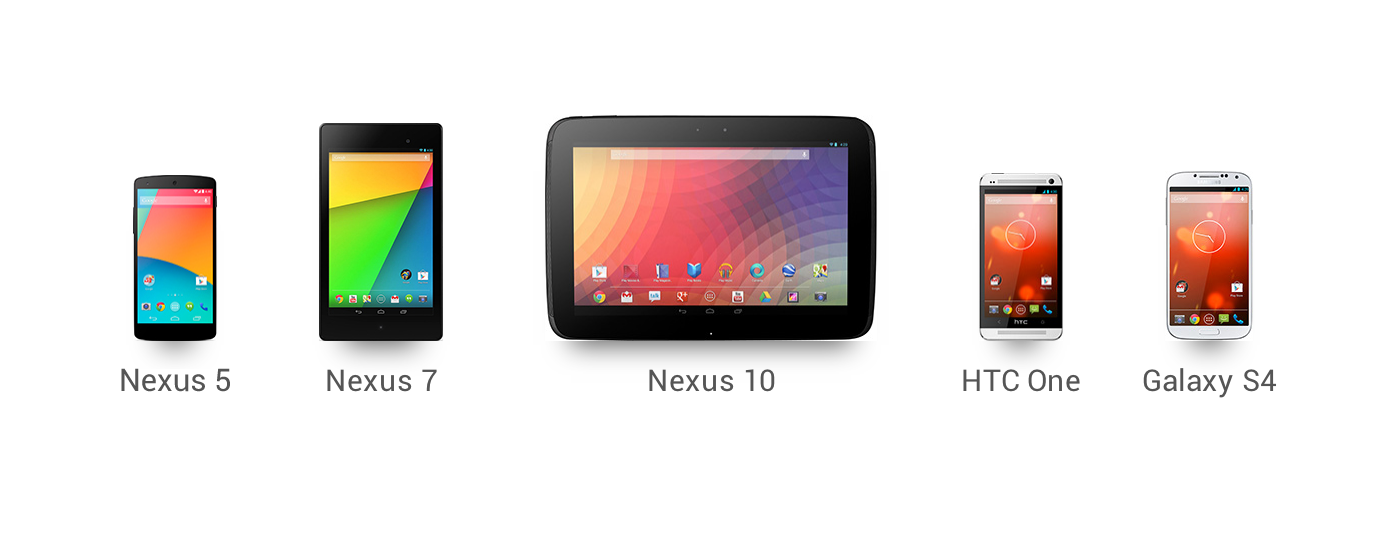
\includegraphics[width=12cm]{Imagenes/dispositivos_android}
\caption{�ltimos smartphones y tablets destacadas en el sitio de Android.}
\label{fig:Fig2}
\end{figure}

A continuaci�n se listan los otros dispositivos que cuentan con Android:
\begin{itemize}
\item Lectores de libros.

\item C�maras.

\item Sistemas en veh�culos.

\item Casas inteligentes.

\item Consolas de videojuegos.

\item Televisores inteligentes.

\item Relojes inteligentes.
\end{itemize}

\subsection{Versiones}
En la figura \ref{fig:Fig3} se detallan las distintas versiones que ha tenido Android. La primera versi�n comercial fue lanzada en Septiembre del 2008. Android est� bajo constante desarrollo por parte de Google y de la Open Handset Alliance, contando con un gran n�mero de actualizaciones desde su lanzamiento.\\
\par
Desde Abril del 2009, los nombres de las versiones de Android han estado relacionados con postres y dulces, y adem�s han seguido un orden alfab�tico. El oreden es Cupcake (1.5), Donut (1.6), Eclair (2.0-2.1), Froyo (2.2-2.2.3), Gingerbread (2.3-2.3.7), Honeycomb (3.0-3.2.5), Ice Cream Sandwich (4.0-4.0.4), Jelly Bean (4.1-4.3), y KitKat(4.4). El 3 de Septiembre del 2013, Google anunci� que exist�an un bill�n de dispositivos activos usando el sistema operativo Android en todo el mundo. La actualizaci�n m�s reciente de android fue KitKat 4.4, el cual fue lanzado para dispositivos comerciales el 22 de Noviembre del 2013.
\begin{figure}[h!]
\centering
	    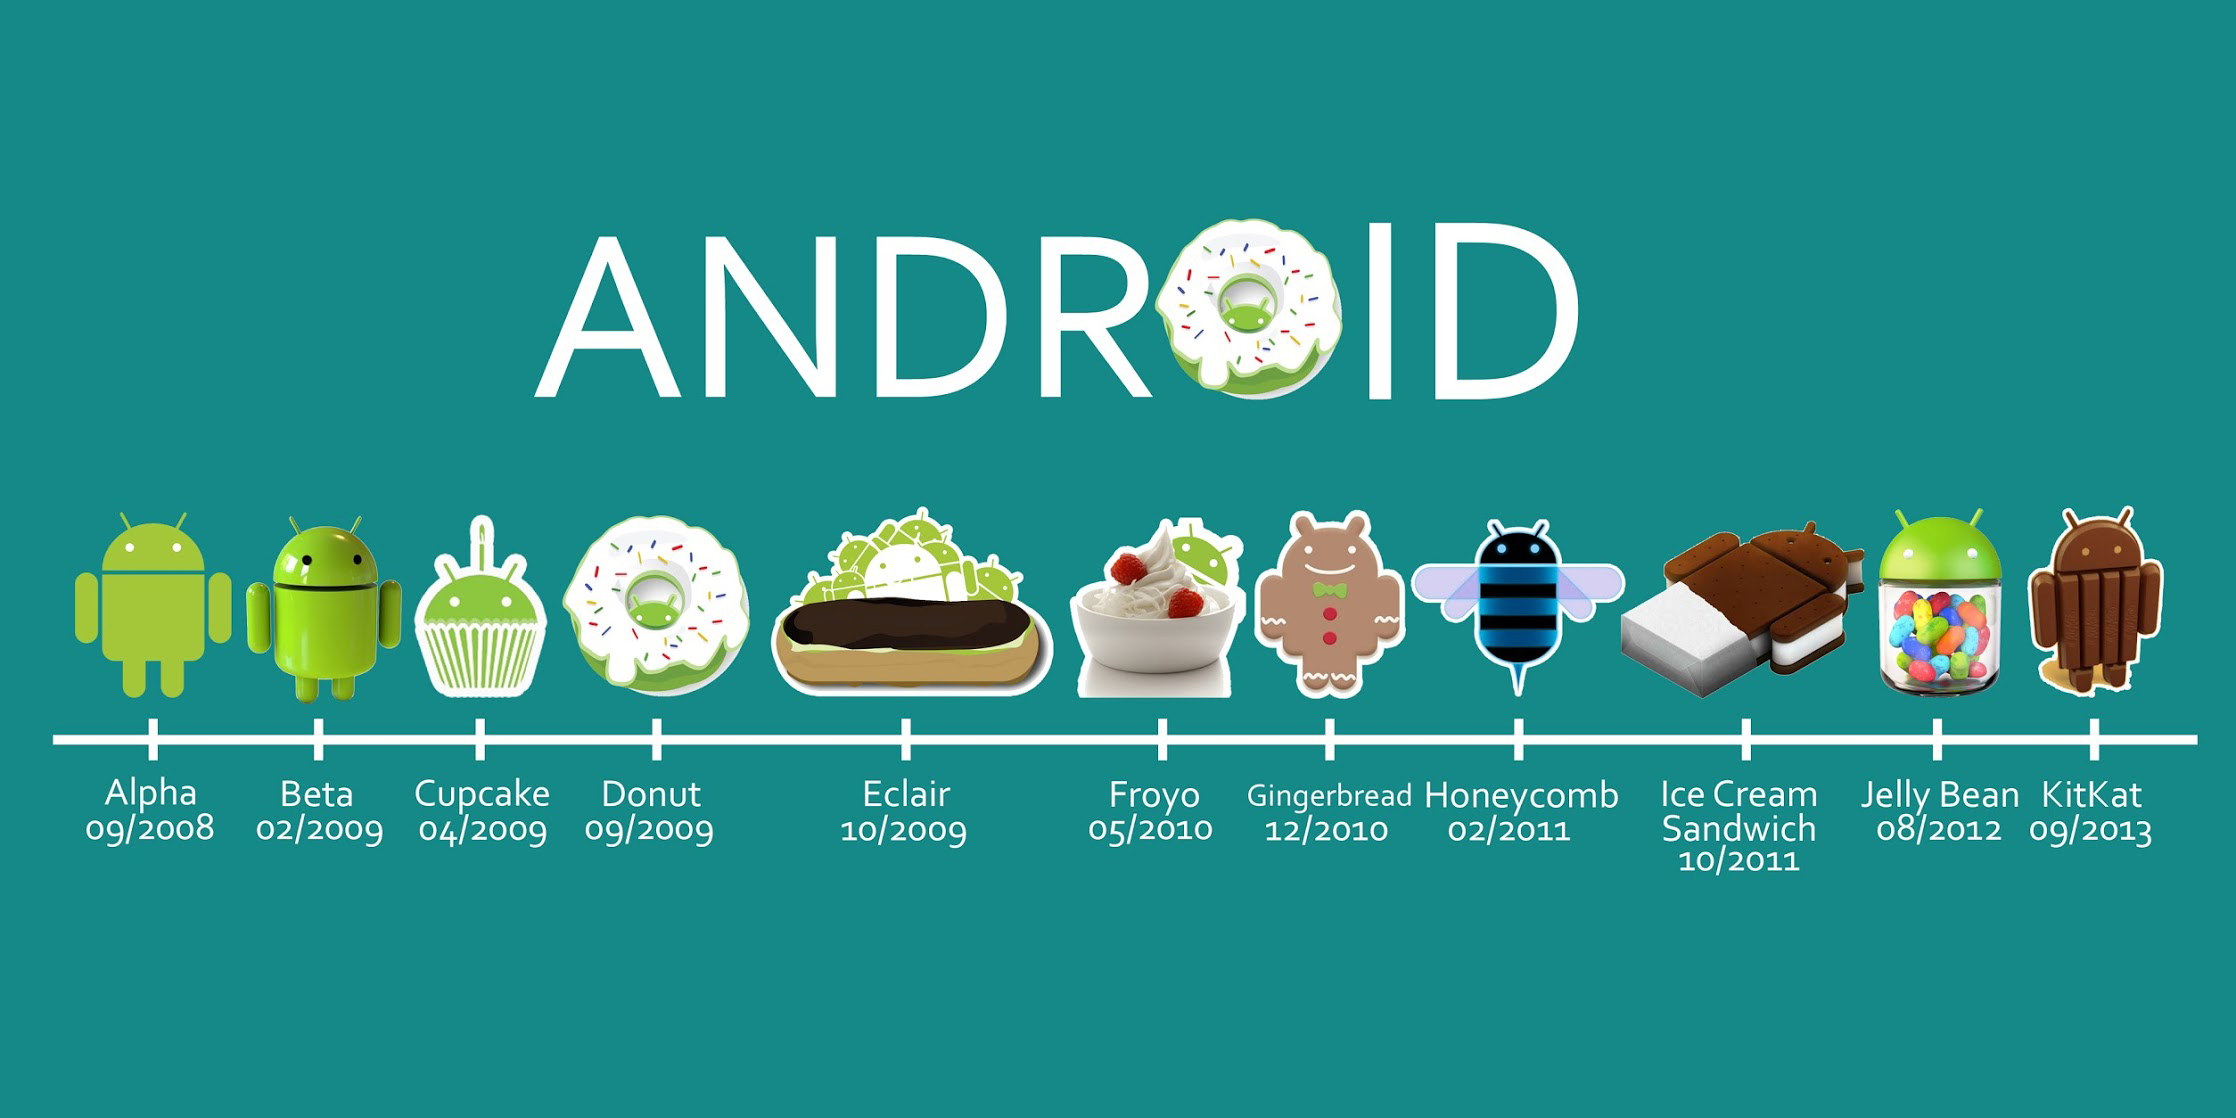
\includegraphics[width=12cm]{Imagenes/versiones_android}
\caption{Versiones de Android.}
\label{fig:Fig3}
\end{figure}

Al comenzar el desarrollo de una aplicaci�n Android, se debe decidir cual va a ser la API m�nima a la cu�l se dar� soporte. Esto tendr� repercusiones al momento de que un usuario desee instalar la aplicaci�n, ya que si su dispositivo cuenta con una versi�n como Froyo o Eclair, lo m�s probable es que no pueda instalar pr�cticamente ning�na de las aplicaciones disponibles en Google Play, la tienda en que se encuentran todas las aplicaciones que suben los desarrolladores.\\
\par
Android actualiza mes a mes las estad�sticas relativas al n�mero de dispositivos que tienen cada versi�n del sistema operativo \cite{2}. Esto ayuda a tener una gu�a sobre cu�l va a ser la API m�nima soportada. En la figura \ref{fig:Fig4} se muestran las estad�sticas correspondientes al mes de Abril. Esta informaci�n es recolectada durante los �ltimos 7 d�as de cada mes, terminando el 1 de Abril del 2014. Adem�s se ignoran las versiones que tienen menos de un 0.1\%. Se puede apreciar que el sistema operativo que hoy en d�a es dominante corresponde a Jelly Bean con m�s de un 60\%. El nuevo sistema operativo KitKat tiene s�lo un 5.3\% debido principalmente a que los operadores y fabricantes a�n no tienen listas sus versiones personalizadas de KitKat, en las que pueden incluir nuevas funcionalidades o quitar lo que estimen conveniente.
\begin{figure}[h!]
\centering
	    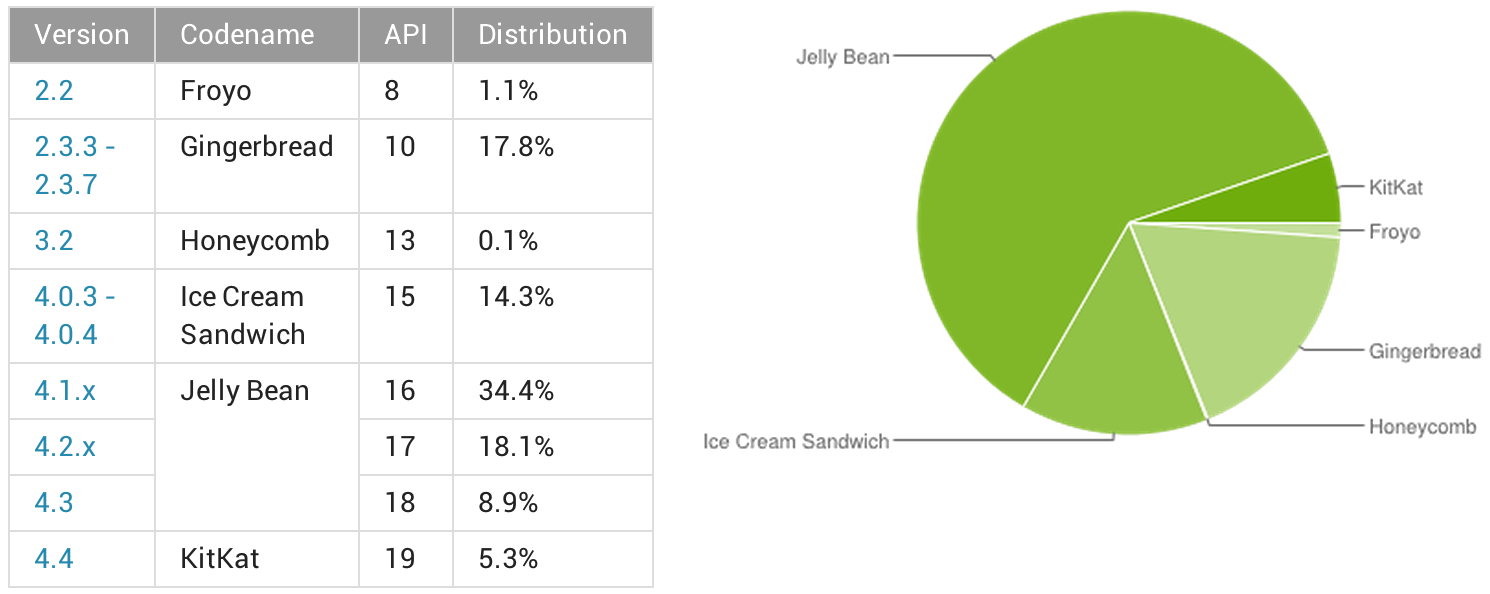
\includegraphics[width=12cm]{Imagenes/dashboard_android}
\caption{Estad�sticas relativas al n�mero de dispositivos que tiene cada versi�n de Android en Abril del 2014.}
\label{fig:Fig4}
\end{figure}


\section{Problemas al desarrollar en Android}
Ahora que ya se han dado a conocer aspectos b�sicos sobre Android, se puede profundizar en los problemas m�s com�nes que se enfrentan al desarrollar aplicaciones.

\subsection{Fragmentaci�n a nivel de software}
Como ya se mencion� anteriormente, existen muchos sistemas operativos de Android vigentes hoy en d�a. Esto priva al desarrollador de muchos funciones �tiles al momento de programar su aplicaci�n, ya que se debe establecer una API m�nima. En base a las estad�sticas que provee Android, la mayor�a de los desarrolladores decide dar soporte desde Gingerbread en adelante. Si el desarrollador desea utilizar m�todos de una API superior a la de Gingerbread, debe especificar en el c�digo fuente que esa parte s�lo tiene que ser ejecutada si el dispositivo del usuario es mayor o igual a la API 11. La siguiente porci�n de c�digo es un ejemplo de lo que los desarrolladores deben hacer: \\
\begin{lstlisting}
if (Build.VERSION.SDK_INT > Build.VERSION_CODES.GINGERBREAD_MR1) {
    // Aqu� va c�digo superior a la API 10 de Gingerbread
}
\end{lstlisting}
Esto provoca que muchas veces el desarrollador deba programar una funcionalidad m�s de una vez. Actualmente muchos desarrolladores est�n optando por dar soporte a sus aplicaciones desde Ice Cream Sandwich en adelante, debido principalmente a la gran recepci�n que ha tenido Jelly Bean y a la ca�da constante que est� teniendo Gingerbread. Si se toma en cuenta que este �ltimo sistema operativo fue lanzado el a�o 2010 y a�n cuenta con cerca de un 20\%, se puede apreciar claramente el nivel de fragmentaci�n que existe, principalmente por la r�pidez con la que Android ha estado mejorando su sistema operativo, lanzando aproximadamente una nueva versi�n cada a�o. \\
\par
A continuaci�n, en el gr�fico de la figura \ref{fig:Fig5} se puede ver la distribuci�n hist�rica de versiones que ha tenido Android con el pasar de los a�os. Si bien se puede ver que a�n existe una gran fragmentaci�n, esto ha ido disminuyendo y Android cada vez se est� convirtiendo en un sistema operativo m�s estable y maduro. Por ejemplo, si se compara el porcentaje que ten�a Gingerbread en el a�o 2013 (39.8\%) con el de este a�o (17.8\%) se ve que hay una diferencia sustancial, y gran parte de este porcentaje se ha trasladado a Jelly Bean, que el a�o pasado contaba con un 25\% del mercado y hoy en d�a cuenta con m�s del 60\%. \\
\begin{figure}[h!]
\centering
	    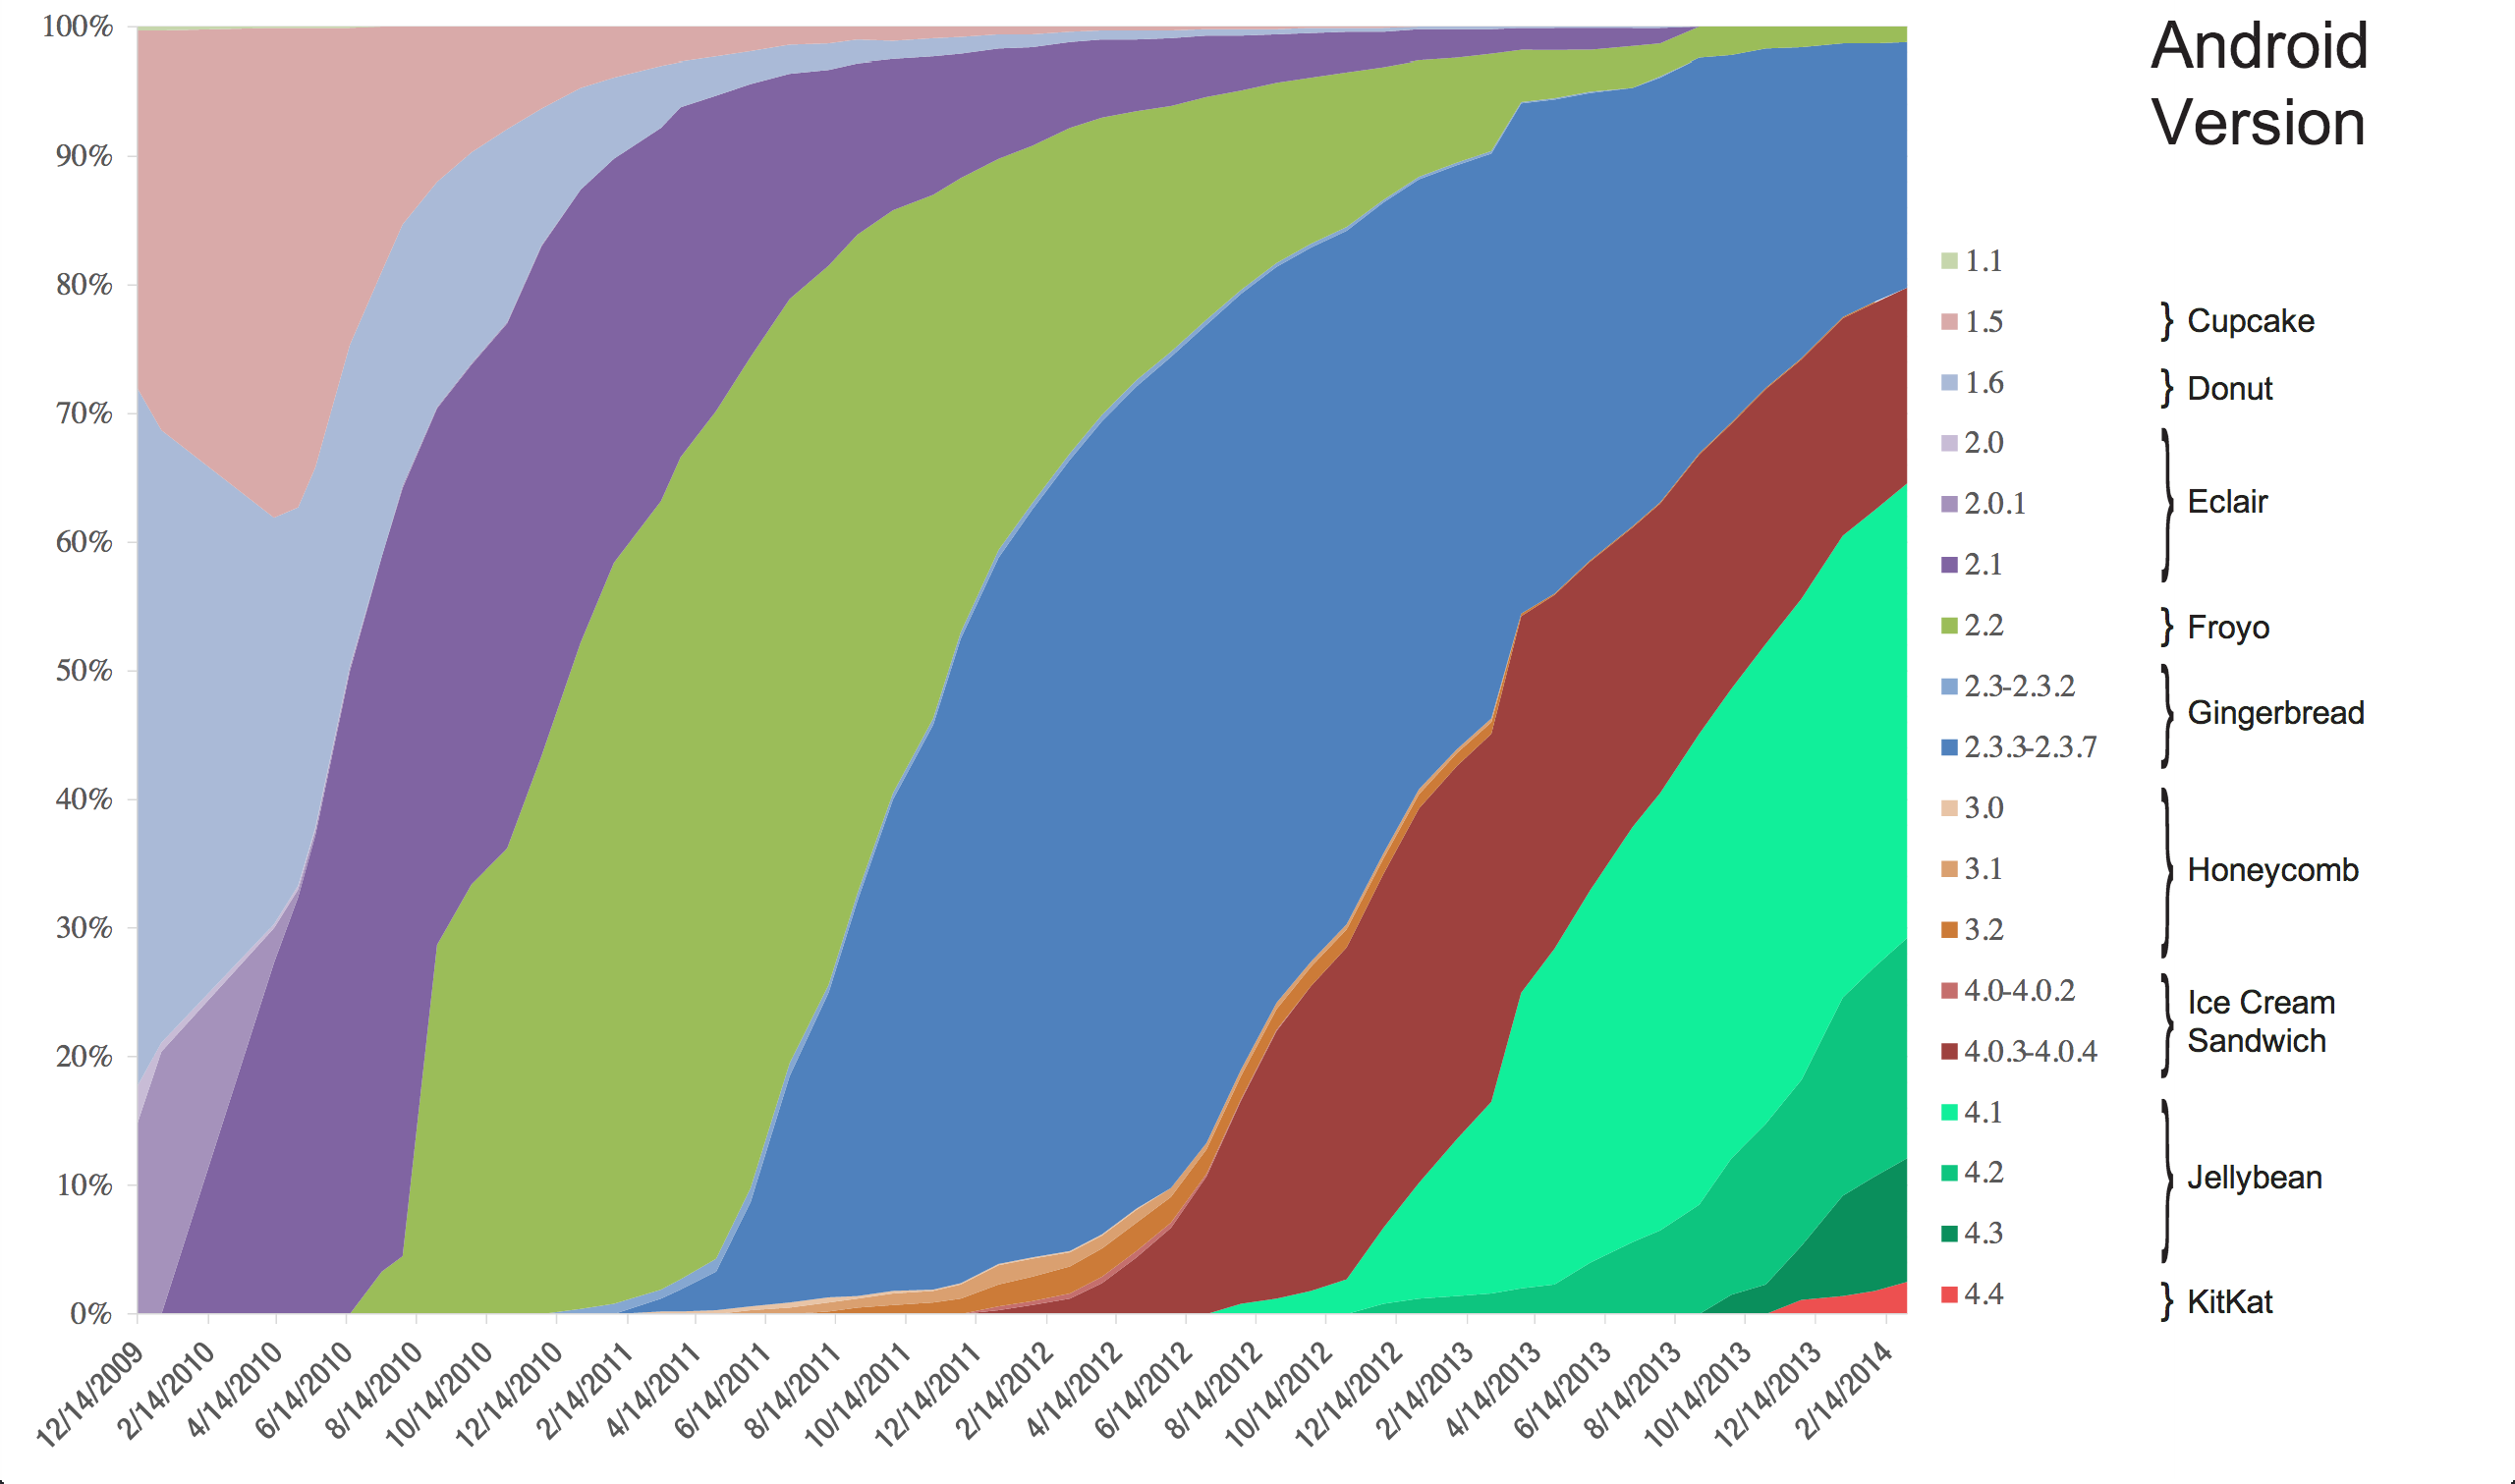
\includegraphics[width=12cm]{Imagenes/historical_progress_android}
\caption{Distribuci�n historica de versiones de Android}
\label{fig:Fig5}
\end{figure}
\par
Muchas veces los crashes y errores en los que la aplicaci�n deja de funcionar correctamente, ocurren en un sistema operativo m�s antiguo y ya fueron arreglados en los sistemas operativos m�s nuevos. Esto ocasiona que al probar la aplicaci�n en un smartphone como un Nexus 4 o como un Samsung S3 no ocurran problemas que si podr�an verse en dispositivos m�s antiguos.  Adem�s, debido a que a veces los operadores o fabricantes no ofrecen actualizaciones al sistema actual, el dispositivo no es actualizado, por lo que estos errores persistir�n.

\subsection{Fragmentaci�n a nivel de hardware}
Aqu� existe fragmentaci�n en muchos sentidos, por un lado tenemos los tama�os de pantalla distintos, las resoluciones de pantalla distintas. Por otro lado hay que considerar que cada dispositivo tiene una cantidad de espacio y memoria distintos, como tambi�n que algunos pueden tener un teclado f�sico, puede que no tengan c�mara, etc. Por �ltimo, muchas veces los fabricantes como Samsung, hacen cambios en el sistema operativo, cambiando cosas nativas, lo cu�l produce diferentes experiencias en cada dispositivo, y muchas veces genera errores que no son culpa del desarrollador.

Lorem ipsum ad his scripta blandit partiendo, eum fastidii accumsan euripidis in, eum liber hendrerit an. Qui ut wisi vocibus suscipiantur, quo dicit ridens inciderint id. Quo mundi lobortis reformidans eu, legimus senserit definiebas an eos. Eu sit tincidunt incorrupte definitionem, vis mutat affert percipit cu, eirmod consectetuer signiferumque eu per. In usu latine equidem dolores. Quo no falli viris intellegam, ut fugit veritus placerat per.

\subsection{Otros problemas}
Lorem ipsum ad his scripta blandit partiendo, eum fastidii accumsan euripidis in, eum liber hendrerit an. Qui ut wisi vocibus suscipiantur, quo dicit ridens inciderint id. Quo mundi lobortis reformidans eu, legimus senserit definiebas an eos. Eu sit tincidunt incorrupte definitionem, vis mutat affert percipit cu, eirmod consectetuer signiferumque eu per. In usu latine equidem dolores. Quo no falli viris intellegam, ut fugit veritus placerat per.


   



\newpage{\pagestyle{empty}\cleardoublepage}

\chapter{Herramientas Actuales}

Lorem ipsum ad his scripta blandit partiendo, eum fastidii accumsan euripidis in, eum liber hendrerit an. Qui ut wisi vocibus suscipiantur, quo dicit ridens inciderint id. Quo mundi lobortis reformidans eu, legimus senserit definiebas an eos. Eu sit tincidunt incorrupte definitionem, vis mutat affert percipit cu, eirmod consectetuer signiferumque eu per. In usu latine equidem dolores. Quo no falli viris intellegam, ut fugit veritus placerat per.

\section{Herramientas de Testing}
Lorem ipsum ad his scripta blandit partiendo, eum fastidii accumsan euripidis in, eum liber hendrerit an. Qui ut wisi vocibus suscipiantur, quo dicit ridens inciderint id. Quo mundi lobortis reformidans eu, legimus senserit definiebas an eos. Eu sit tincidunt incorrupte definitionem, vis mutat affert percipit cu, eirmod consectetuer signiferumque eu per. In usu latine equidem dolores. Quo no falli viris intellegam, ut fugit veritus placerat per.\\
\textbf{DIVIDIR ENTRE DISTINTOS TIPOS DE TESTING}

\subsection{JUnit}
Lorem ipsum ad his scripta blandit partiendo, eum fastidii accumsan euripidis in, eum liber hendrerit an. Qui ut wisi vocibus suscipiantur, quo dicit ridens inciderint id. Quo mundi lobortis reformidans eu, legimus senserit definiebas an eos. Eu sit tincidunt incorrupte definitionem, vis mutat affert percipit cu, eirmod consectetuer signiferumque eu per. In usu latine equidem dolores. Quo no falli viris intellegam, ut fugit veritus placerat per.

\subsection{EasyMock}
Lorem ipsum ad his scripta blandit partiendo, eum fastidii accumsan euripidis in, eum liber hendrerit an. Qui ut wisi vocibus suscipiantur, quo dicit ridens inciderint id. Quo mundi lobortis reformidans eu, legimus senserit definiebas an eos. Eu sit tincidunt incorrupte definitionem, vis mutat affert percipit cu, eirmod consectetuer signiferumque eu per. In usu latine equidem dolores. Quo no falli viris intellegam, ut fugit veritus placerat per.

\subsection{PowerMock}
Lorem ipsum ad his scripta blandit partiendo, eum fastidii accumsan euripidis in, eum liber hendrerit an. Qui ut wisi vocibus suscipiantur, quo dicit ridens inciderint id. Quo mundi lobortis reformidans eu, legimus senserit definiebas an eos. Eu sit tincidunt incorrupte definitionem, vis mutat affert percipit cu, eirmod consectetuer signiferumque eu per. In usu latine equidem dolores. Quo no falli viris intellegam, ut fugit veritus placerat per.

\subsection{Mockito}
Lorem ipsum ad his scripta blandit partiendo, eum fastidii accumsan euripidis in, eum liber hendrerit an. Qui ut wisi vocibus suscipiantur, quo dicit ridens inciderint id. Quo mundi lobortis reformidans eu, legimus senserit definiebas an eos. Eu sit tincidunt incorrupte definitionem, vis mutat affert percipit cu, eirmod consectetuer signiferumque eu per. In usu latine equidem dolores. Quo no falli viris intellegam, ut fugit veritus placerat per.

\subsection{Espresso}
Lorem ipsum ad his scripta blandit partiendo, eum fastidii accumsan euripidis in, eum liber hendrerit an. Qui ut wisi vocibus suscipiantur, quo dicit ridens inciderint id. Quo mundi lobortis reformidans eu, legimus senserit definiebas an eos. Eu sit tincidunt incorrupte definitionem, vis mutat affert percipit cu, eirmod consectetuer signiferumque eu per. In usu latine equidem dolores. Quo no falli viris intellegam, ut fugit veritus placerat per.

\subsection{Robotium}
Lorem ipsum ad his scripta blandit partiendo, eum fastidii accumsan euripidis in, eum liber hendrerit an. Qui ut wisi vocibus suscipiantur, quo dicit ridens inciderint id. Quo mundi lobortis reformidans eu, legimus senserit definiebas an eos. Eu sit tincidunt incorrupte definitionem, vis mutat affert percipit cu, eirmod consectetuer signiferumque eu per. In usu latine equidem dolores. Quo no falli viris intellegam, ut fugit veritus placerat per.

\subsection{Robolectric}
Lorem ipsum ad his scripta blandit partiendo, eum fastidii accumsan euripidis in, eum liber hendrerit an. Qui ut wisi vocibus suscipiantur, quo dicit ridens inciderint id. Quo mundi lobortis reformidans eu, legimus senserit definiebas an eos. Eu sit tincidunt incorrupte definitionem, vis mutat affert percipit cu, eirmod consectetuer signiferumque eu per. In usu latine equidem dolores. Quo no falli viris intellegam, ut fugit veritus placerat per.

\subsection{Spoon}
Lorem ipsum ad his scripta blandit partiendo, eum fastidii accumsan euripidis in, eum liber hendrerit an. Qui ut wisi vocibus suscipiantur, quo dicit ridens inciderint id. Quo mundi lobortis reformidans eu, legimus senserit definiebas an eos. Eu sit tincidunt incorrupte definitionem, vis mutat affert percipit cu, eirmod consectetuer signiferumque eu per. In usu latine equidem dolores. Quo no falli viris intellegam, ut fugit veritus placerat per.

\section{Herramientas de Crashes}
Lorem ipsum ad his scripta blandit partiendo, eum fastidii accumsan euripidis in, eum liber hendrerit an. Qui ut wisi vocibus suscipiantur, quo dicit ridens inciderint id. Quo mundi lobortis reformidans eu, legimus senserit definiebas an eos. Eu sit tincidunt incorrupte definitionem, vis mutat affert percipit cu, eirmod consectetuer signiferumque eu per. In usu latine equidem dolores. Quo no falli viris intellegam, ut fugit veritus placerat per.

\subsection{Crittercism}
Lorem ipsum ad his scripta blandit partiendo, eum fastidii accumsan euripidis in, eum liber hendrerit an. Qui ut wisi vocibus suscipiantur, quo dicit ridens inciderint id. Quo mundi lobortis reformidans eu, legimus senserit definiebas an eos. Eu sit tincidunt incorrupte definitionem, vis mutat affert percipit cu, eirmod consectetuer signiferumque eu per. In usu latine equidem dolores. Quo no falli viris intellegam, ut fugit veritus placerat per.

\subsection{Bugsense}
Lorem ipsum ad his scripta blandit partiendo, eum fastidii accumsan euripidis in, eum liber hendrerit an. Qui ut wisi vocibus suscipiantur, quo dicit ridens inciderint id. Quo mundi lobortis reformidans eu, legimus senserit definiebas an eos. Eu sit tincidunt incorrupte definitionem, vis mutat affert percipit cu, eirmod consectetuer signiferumque eu per. In usu latine equidem dolores. Quo no falli viris intellegam, ut fugit veritus placerat per.

\subsection{Crashlytics}
Lorem ipsum ad his scripta blandit partiendo, eum fastidii accumsan euripidis in, eum liber hendrerit an. Qui ut wisi vocibus suscipiantur, quo dicit ridens inciderint id. Quo mundi lobortis reformidans eu, legimus senserit definiebas an eos. Eu sit tincidunt incorrupte definitionem, vis mutat affert percipit cu, eirmod consectetuer signiferumque eu per. In usu latine equidem dolores. Quo no falli viris intellegam, ut fugit veritus placerat per.

\subsection{ACRA}
Lorem ipsum ad his scripta blandit partiendo, eum fastidii accumsan euripidis in, eum liber hendrerit an. Qui ut wisi vocibus suscipiantur, quo dicit ridens inciderint id. Quo mundi lobortis reformidans eu, legimus senserit definiebas an eos. Eu sit tincidunt incorrupte definitionem, vis mutat affert percipit cu, eirmod consectetuer signiferumque eu per. In usu latine equidem dolores. Quo no falli viris intellegam, ut fugit veritus placerat per.

\subsection{Google Analytics}
Lorem ipsum ad his scripta blandit partiendo, eum fastidii accumsan euripidis in, eum liber hendrerit an. Qui ut wisi vocibus suscipiantur, quo dicit ridens inciderint id. Quo mundi lobortis reformidans eu, legimus senserit definiebas an eos. Eu sit tincidunt incorrupte definitionem, vis mutat affert percipit cu, eirmod consectetuer signiferumque eu per. In usu latine equidem dolores. Quo no falli viris intellegam, ut fugit veritus placerat per.



\newpage{\pagestyle{empty}\cleardoublepage}

\chapter{An�lisis Comparativo}

Para este an�lisis comparativo hemos filtrado las aplicaciones que pueden ser m�s �tiles y que pueden ser comparadas, ya que muchas de las herramientas estudiadas son muy distintas una de otra, por lo que es muy complicado realizar una comparaci�n.

Sed iusto nihil populo an, ex pro novum homero cotidieque. Te utamur civibus eleifend qui, nam ei brute doming concludaturque, modo aliquam facilisi nec no. Vidisse maiestatis constituam eu his, esse pertinacia intellegam ius cu. Eos ei odio veniam, eu sumo altera adipisci eam, mea audiam prodesset persequeris ea. Ad vitae dictas vituperata sed, eum posse labore postulant id. Te eligendi principes dignissim sit, te vel dicant officiis repudiandae.

Id vel sensibus honestatis omittantur, vel cu nobis commune patrioque. In accusata definiebas qui, id tale malorum dolorem sed, solum clita phaedrum ne his. Eos mutat ullum forensibus ex, wisi perfecto urbanitas cu eam, no vis dicunt impetus. Assum novum in pri, vix an suavitate moderatius, id has reformidans referrentur. Elit inciderint omittantur duo ut, dicit democritum signiferumque eu est, ad suscipit delectus mandamus duo. An harum equidem maiestatis nec.
At has veri feugait placerat, in semper offendit praesent his. Omnium impetus facilis sed at, ex viris tincidunt ius. Unum eirmod dignissim id quo. Sit te atomorum quaerendum neglegentur, his primis tamquam et. Eu quo quot veri alienum, ea eos nullam luptatum accusamus. Ea mel causae phaedrum reprimique, at vidisse dolores ocurreret nam. 

\newpage{\pagestyle{empty}\cleardoublepage}

\chapter{Implementaci�n en entorno real}

Sed iusto nihil populo an, ex pro novum homero cotidieque. Te utamur civibus eleifend qui, nam ei brute doming concludaturque, modo aliquam facilisi nec no. Vidisse maiestatis constituam eu his, esse pertinacia intellegam ius cu. Eos ei odio veniam, eu sumo altera adipisci eam, mea audiam prodesset persequeris ea. Ad vitae dictas vituperata sed, eum posse labore postulant id. Te eligendi principes dignissim sit, te vel dicant officiis repudiandae.

Id vel sensibus honestatis omittantur, vel cu nobis commune patrioque. In accusata definiebas qui, id tale malorum dolorem sed, solum clita phaedrum ne his. Eos mutat ullum forensibus ex, wisi perfecto urbanitas cu eam, no vis dicunt impetus. Assum novum in pri, vix an suavitate moderatius, id has reformidans referrentur. Elit inciderint omittantur duo ut, dicit democritum signiferumque eu est, ad suscipit delectus mandamus duo. An harum equidem maiestatis nec.
At has veri feugait placerat, in semper offendit praesent his. Omnium impetus facilis sed at, ex viris tincidunt ius. Unum eirmod dignissim id quo. Sit te atomorum quaerendum neglegentur, his primis tamquam et. Eu quo quot veri alienum, ea eos nullam luptatum accusamus. Ea mel causae phaedrum reprimique, at vidisse dolores ocurreret nam. 

\newpage{\pagestyle{empty}\cleardoublepage}

\chapter{Conclusi�n}

Sed iusto nihil populo an, ex pro novum homero cotidieque. Te utamur civibus eleifend qui, nam ei brute doming concludaturque, modo aliquam facilisi nec no. Vidisse maiestatis constituam eu his, esse pertinacia intellegam ius cu. Eos ei odio veniam, eu sumo altera adipisci eam, mea audiam prodesset persequeris ea. Ad vitae dictas vituperata sed, eum posse labore postulant id. Te eligendi principes dignissim sit, te vel dicant officiis repudiandae.

Id vel sensibus honestatis omittantur, vel cu nobis commune patrioque. In accusata definiebas qui, id tale malorum dolorem sed, solum clita phaedrum ne his. Eos mutat ullum forensibus ex, wisi perfecto urbanitas cu eam, no vis dicunt impetus. Assum novum in pri, vix an suavitate moderatius, id has reformidans referrentur. Elit inciderint omittantur duo ut, dicit democritum signiferumque eu est, ad suscipit delectus mandamus duo. An harum equidem maiestatis nec.
At has veri feugait placerat, in semper offendit praesent his. Omnium impetus facilis sed at, ex viris tincidunt ius. Unum eirmod dignissim id quo. Sit te atomorum quaerendum neglegentur, his primis tamquam et. Eu quo quot veri alienum, ea eos nullam luptatum accusamus. Ea mel causae phaedrum reprimique, at vidisse dolores ocurreret nam. 

%Bibliografia

\bibliographystyle{plain}
\bibliography{bib_TI}

\listoffigures

\end{document} 